\chapter{Resilience}
\index{Resilience@\emph{Resilience}}%
\section{Introduction}
Given that we have constructed models for response to a scenario of a hurricane strike on power and road infrastructures, we can use these to look at how different methods of resilience interact with repair. We define resilience as the ability to withstand disruption and efficiently return to normal operation, but there are many definitions of resilience throughout literature on network operations \cite{MolyneauxEA2016}. In this chapter, we consider increasing the grid's resilience through hardening and fortification rather than an islanding based approach. We can then look to the repair procedures to evaluate the resilience of the power grid through looking at the rate of repair rather than just looking at the time to resume normal operation or magnitude of maximum initial drop in performance.

Most approaches to resilience construct a resilience curve such as the one in Figure 4.1  taken from \cite{Madni2020}. Resilience is shown as an initial drop and then time to both partial and full recovery.

\begin{figure}[htbp]
	\centering
	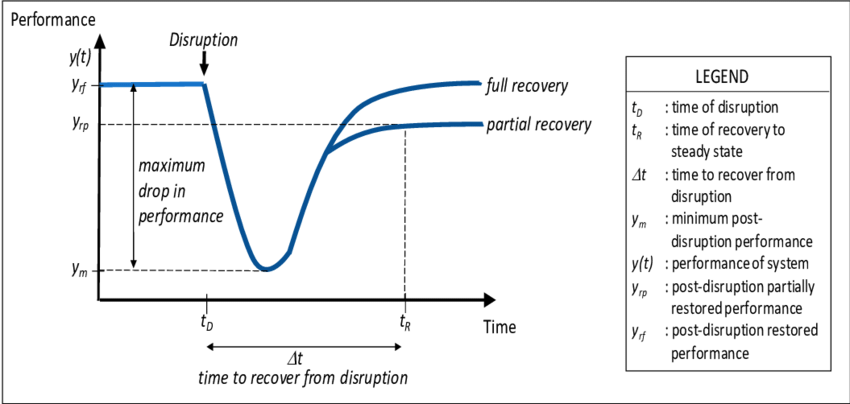
\includegraphics[width=.9\linewidth]{resiliencecurve.png}
	\caption{Standard depiction of a resilience curve}
\end{figure}

Large sections of the literature assume the recovery process for a system is fixed, so they study resilience in the context of minimizing either time to restoration of nominal system performance or minimizing the magnitude of the initial drop. We can frame this in terms of looking at the means versus the end. The goal is not to minimize some metric of resilience, but rather to reduce the impact of damage to the power grid. As we have been working with models for repair of damaged networks that generate repair schedules and associated curves showing power demand shed over time, we can look at all aspects of the resilience curve. This method gives us both the magnitude of the initial drop and the time to recovery in addition to the repair curve generated. Using this, we look into how the repair model defined above interacts with standard methods of improving resilience of a power grid.

\section{Hardening}

Hardening is one of the approaches to resilience achieved by fortifying a subset of nodes and edges in a network to make the network harder to damage. In the context of a power grid, this can include placing additional support guide wires on power poles, burying lines, or building flood walls and windbreakers around substations. Hardening is often looked at in the context of interdiction problems \cite{ChurchEA2007}.

 To overview the problem solved in interdiction: player 1 operates a network, player 2 attacks the network with the objective of maximizing demand shed under optimal power grid operation, and player 1 hardens the network before the attack under the assumption that it is coming and wants to preserve as much of the network's capacity as possible given a budget for hardening. This can be formulated as a trilayer maximization/minimization/maximization mixed integer programming \cite{Mahmoo2016}. Alternatively, it can be approached as a stochastic problem with uncertainties used to model attacks not being guaranteed to succeed \cite{Ramirez2009}.

A similar approach can be taken with disaster planning. Unlike in interdiction, the attack coming from a hurricane is a semi-random process of nature and not a targeted interdiction by an intelligent actor. Therefore the exact methods from directed attack based interdiction can not be implemented for models with more layers of decisions past attack and hardening. When solving this problem, we find a fixed quantity of damage based on the amount of hardening that can be undertaken with a budget constraint. By solving the ensuing interdiction problem, choosing the combination of elements that would be damaged forms the best set of elements to harden against damage. Solving this to optimality with best practices requires a delve into bi-level optimization that is outside the scope of this thesis. We therefore solve the problem heuristically through the following setup.

\begin{enumerate}
	
	\item Solve the baseline DC-OPF model for the given power grid
	\item Identify how many nodes (N) and edges (E) that are to be hardened based on the budget constraint
	\item Select at least the 2N highest demand nodes and the 2E highest utilization edges based on the DC-OPF model
	\item For each possible subset of N nodes and E edges, solve DC-OPF with those elements damaged (i.e down)
	\item Out of all the tested subsets, find the one that produces the maximum load shed in the DC-OPF solution. Use that subset of nodes and edges as the best choice for hardening when analyzing resilience.
\end{enumerate}

This is a heuristic solution rather than guaranteed optimality as written. In the case where all possible subsets are considered, this method generates a full solution to the multilayer (maximization of the minimum) optimization problem through enumeration. The result of this is a set of power grid elements that, if damaged, would maximally impede the operation of the power grid. The implication then is that by protecting this set of elements, the grid would be best protected against the worst case. This is the approach that Salmeron et al. \cite{Salmeron2004} took when studying terror attacks in the context of power grid resilience.
\section{Modeling}
We elect to use the IEEE 30 bus network outlined in earlier chapters to demonstrate the effectiveness of interdiction and priority heuristic based resilience procedure. Each scenario is solved three times using the interaction framework of solving the road grid first and then solving power grid repair based on that road repair schedule as laid out in Chapters 2 and 3. We solve for resilience in three ways:
\begin{itemize}
	\item Choosing hardened elements based on the interdiction method defined above
	\item Choosing hardened elements heuristically where the highest demand nodes and the edges that have the highest ratio of flow compared to their maximum flow limit. This is the kind of approximation that a power utility may use to choose elements to harden.
	\item Choosing no elements to be hardened
\end{itemize}.


Solution for the interdiction based hardening is done to optimality by selecting every subset of the desired size. The runtime for doing this is about 90 minutes because the model for load shed is a linear program and solves efficiently. The literature base on interdiction will have more sophisticated models and metaheuristics to solve or approximate interdiction on larger networks, but they are unnecessary for grids of this size since the optimal solution can be found with this simpler method.

We show the chosen hardened elements in Table 4.1 with the grid topology shown in Figure 4.2 for clarity as to what's hardened. Were all the elements from the interdiction based hardening method to be damaged, $233.4$ MW of demand would have to be shed. For the priority heuristic based method's chosen elements being damaged, the power grid would have to shed $187.6$ MW of demand.
\begin{figure}[htbp]
	\centering
	\includegraphics[width=.75\linewidth]{IEEE30layout.png}
	\caption{Layout of the power grid used for hardening and resilience}
\end{figure}

\begin{table}[htbp]
	\centering
	\caption{Hardened elements by resilience method }
	\resizebox{\columnwidth}{!}{\begin{tabular}{|c|c|c|}
			\hline	
			 & Interdiction Based & Priority Heuristic Based \\\hline
			Nodes & 1 and 7 & 4 and 7\\
			\hline
			Edges & (22,23), (5,9), (1,5), and (0,1)  & (22,23), (5,9), (23,24), and (14,17)\\
			\hline
	\end{tabular}}
	
	\label{time}
\end{table}

 We solve 20 repair problems corresponding to scenarios that are generated by uniform random generation are solved. Each scenario reflects 50\% line loss and 25\% bus loss in the power grid and a standardized road damage of 50\%. We solve the repair problem and find a schedule that will display the difference in not just recovery time, but amount of unsatisfied demand during the repair process for different treatments of resilience. In addition to this, we assess the objective with perfect information to construct a lower bound on the amount of demand unsatisfied in each scenario.

\subsection{Objective with Perfect Information}

 On top of these three methods of comparison in resilience, we also look at a case where we had perfect information about upcoming damage to generate a lower bound to compare to. If we knew which scenario will be realized, then the hardening of the most important elements for that scenario would be the optimal thing to do beforehand. Hardening here occurs with the same budget as the other methods. This method with perfect information is similar to wait-and-see lower bounds in optimization under uncertainty.
 
To assess the objective with perfect information, we construct a simple mixed integer program based on models presented earlier to identify that given we know exactly what damage is about to occur, what elements should be hardened. We formulate it as follows:

\begin{displaymath}
\begin{array}{ll}
N & \mbox{set of nodes, indexed by $i$} \\
E & \mbox{set of power lines, indexed by $e$}\\
O(i) & \mbox{set of lines with origin $i$} \\
D(i) & \mbox{set of lines with destination $i$} \\
o(e) & \mbox{origin node of line $e$} \\
d(e) & \mbox{destination node of line $e$} \\
\underline{L_e},\overline{L_e} & \mbox{power lower and upper bounds for line $e$}\\
D_i & \mbox{power demand in megawatts at node $i$ in the pre-disaster state}\\
P_k & \mbox{maximum power generation in megawatts for the generator at node $k$}\\
B_e &  \mbox{line susceptance in per unit siemens for power line $e$}\\
I_e, I_i & \mbox{a scenario's damage is represented here by $I_e$ and $I_i$ where 1 is working }\\
K_n & \mbox{The maximum number of nodes that can be hardened}\\
K_l & \mbox{The maximum number of edges that can be hardened}\\
X_{e} & \mbox{power flow in megawatts on line $e$}\\
G_{k} & \mbox{production from the generator at node $k$}\\
Y_{n} & \mbox{Load shed in megawatts from bus $n$}\\ 
V_i & \mbox{indicator for node $i$ being operational (1 is working) }\\
W_{e} & \mbox{indicator for line $e$ being operational (1 is working) }\\
U_{e} & \mbox{indicator for line $e$ being chosen to be hardened}\\
F_i & \mbox{indicator for node $i$ being chosen to be hardened}\\
\theta_i & \mbox{phase angle in radians for the power flow at node $i$}\\

\end{array}
\end{displaymath}
\begin{equation}
\textnormal{Minimize} \sum_{i \in N}  Y_i
\end{equation}
\textbf{subject to:}
\begin{eqnarray}
X_e = B_e (\theta_{o(e)} - \theta_{d(e)}),  \hspace{4pt} \forall e \in E\\
G_i - \sum_{e \in O(i)} X_e + \sum_{e \in D(i)} X_e = D_i-Y_i, \hspace{4pt} \forall t \in T, \hspace{4pt} \forall i \in N\\
G_k \leq P_{k} V_{k}, \hspace{4pt} \forall k \in N\\
0\leq Y_i \leq D_i, \hspace{4pt} \forall t \in T, \hspace{4pt} \forall i \in N\\
\underline{L_e}W_{e} \leq X_{e} \leq \overline{L_e}W_{e}, \hspace{4pt} \forall e \in E\\
\underline{L_e}V_{o(e)} \leq X_{e} \leq \overline{L_e}V_{o(e)},  \hspace{4pt} \forall e \in E\\
\underline{L_e}V_{d(e)} \leq X_{e} \leq \overline{L_e}V_{d(e)}, \hspace{4pt} \forall e \in E\\
V_i \leq F_i+I_i, \hspace{4pt} \forall i \in N\\
W_{e} \leq  U_{e}+I_e, \hspace{4pt} \forall e \in E\\
\sum_{i \in N} F_i \leq K_n\\
\sum_{e \in E} U_{e} \leq K_l\\
-\pi/2 \leq \theta_i \leq \pi/2, \hspace{4pt} \forall i \in N\\
S_{e}^t,F_{i}^t,W_{e}^t,V_{i}^t \in \{0,1\}. 
\end{eqnarray}

This is a variation on DC optimal power flow from Chapter 2 with load shedding. The objective is to minimize unsatisfied demand by choosing what elements to harden if we know the exact damage ahead of time. Constraints (4.9-4.12) handle the choice of hardening if the damage to the power grid is known ahead of time. While this is not a problem that will ever occur without weather modeling getting dramatically better, it is useful for generating a lower bound on damage such that a resilience strategy can be compared to both upper (do nothing) and lower (perfect information) bounds.

\section{Results}

We begin by showing the expected load shed across the full suite of 20 scenarios with equal weights on each scenario. We solve this by generating a scenario and computing the set of elements to harden with perfect information. Following this, the repair problem with the road first interaction framework is solved four times corresponding to each method of looking at resilience.  It is worth noting that averaging ``smooths out" the effect of individual scenarios, so several specific scenarios are displayed to make clear what the difference in a single scenario's actualization can be. The averages are shown in Figure 4.3 for hardening of two nodes and four edges.	
\begin{figure}[htbp]
	\centering
	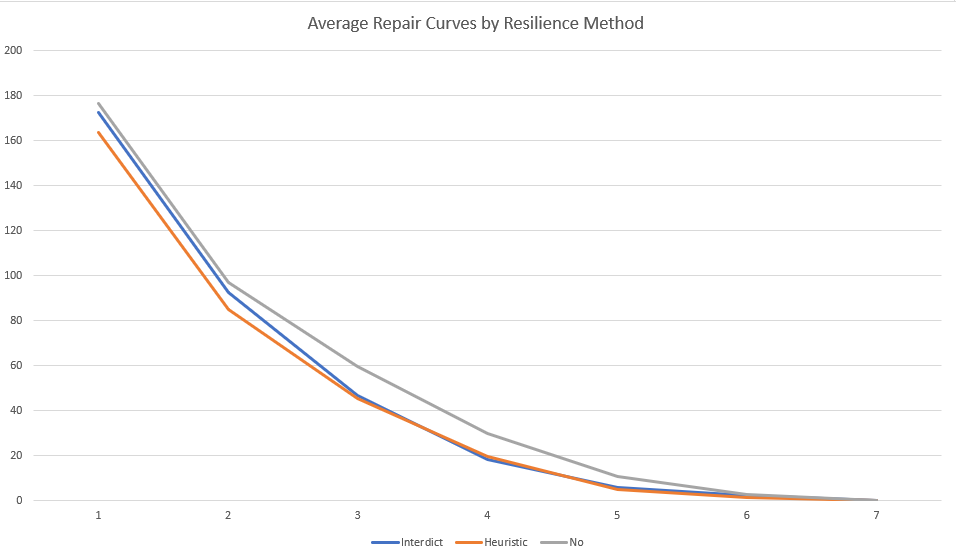
\includegraphics[width=.9\linewidth]{AverageSpaghetti.png}
	\caption{Average load demand shed over the set of 20 random scenarios on IEEE  30 bus}
\end{figure}

\begin{table}[htbp]
	\centering
		\caption{Expected unsatisfied demand by shift in each hardening method}
	\resizebox{\columnwidth}{!}{	\begin{tabular}{|c|c|c|c|c|}	
		\cline{1-5}
		Shift Number & Interdiction Based & Priority Heuristic Based & No Resilience & Perfect Information\\\hline
		1 & 168.3 & 171.5 & 187.9 & 107.4\\\hline
		2 & 74.7 & 92.1 & 100.9 & 39.9\\\hline
		3 & 41.1 & 43.3 & 53.1 & 15.3\\\hline
		4 & 14.8 & 18.3 & 28.3 & 4.54\\\hline
		5 & 4.3 & 4.1 & 9.5 & 0.24\\\hline
		6 & 1.3 & 1 & 2.0 & 0\\\hline
		7 & 0 & 0.12 & 0 & 0\\\hline
		total & 304.7 & 330.4 & 381.8 & 167.3\\\hline
	\end{tabular}}

	\label{time}
\end{table}


When using the interacted models to look at resilience though the repair curve, we find that over the average of the set of random scenarios modeled, interdiction based resilience has lower total expected load shed as well as a smaller expected initial drop. Figure 4.3 provides a visualization of this where the interdiction based method is visibly better than both the heuristic method and doing nothing. Both methods of making the power grid resilient are substantially better than doing nothing as would be intuitively expected, but the difference between use of the priority heuristic and solution to the full interdiction method is much smaller. This is still in line with expectations that more involved modeling should result in a better solution. Table 4.1 shows the direct magnitude where interdiction-based modeling results in the satisfaction of an additional 25 MW-shifts of demand. This small difference is due to interdiction models being best used for planned intelligent attacks and being and imperfect tool for planning hardening for random process.

We then break out the following two specific scenarios to showcase the effect that hardening an element matters most when it would be damaged by the disaster. Figure 4.4 shows the impact of protection of node 4 and several important lines by the priority heuristic based method that were not protected in the interdiction method. In this scenario, node 4 would have been damaged, but wasn't in the priority heuristic method because of hardening. This is not evidence that the heuristic is better than the interdiction method, but it does show the importance of hardening nodes that take damage. By contrast, Figure 4.5 shows a scenario where node 7 would have been damaged, but was not damaged due to hardening in all hardening cases. The differences in repair curves stem from the difference in hardened lines, showing that protection of nodes is not the only factor that matters. 

\begin{figure}[htbp]
	\centering
	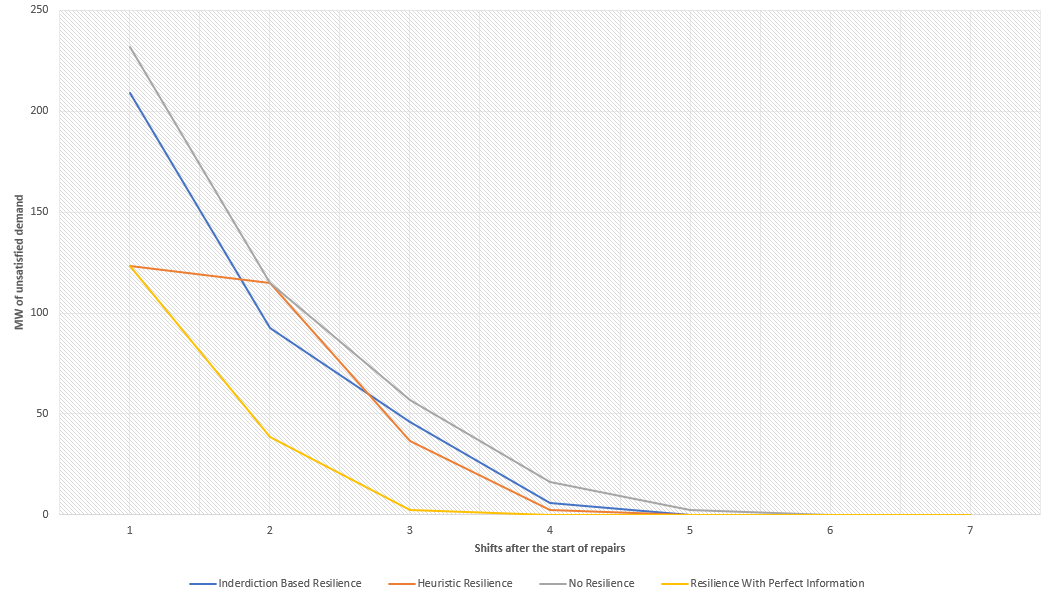
\includegraphics[width=.9\linewidth]{Heuristic24Scenario.png}
	\caption{A specific scenario from resilience modeling that shows the effect of protecting node 4 in the priority heuristic method}
\end{figure}
\begin{figure}[htbp]
	\centering
	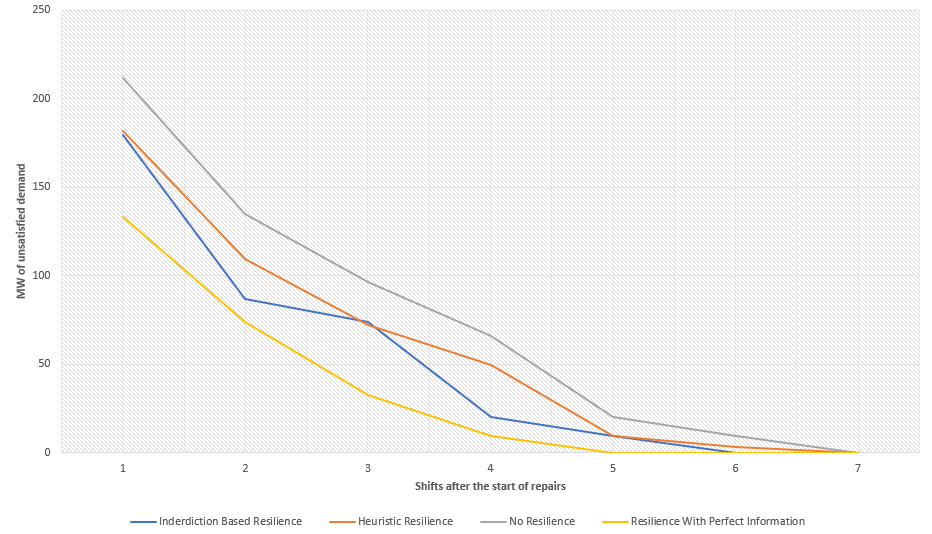
\includegraphics[width=.9\linewidth]{Inderdiction24Scenario.png}
	\caption{A specific scenario from resilience modeling that shows the effect of protecting damaged lines in the interdiction based method}
\end{figure}

Out of concern that the earlier results could be anomalous due to the budget constraint or grid topology based on choices of what elements to fortify, we repeat the process under a different budget constraint. We elect this time to fortify only one node and three edges to show the impact of a reduced budget. In the interdiction based method, we choose node 1 and edges (1,5), (22,23), and (0,1) for the interdiction based hardening. The priority heuristic hardens node 4 and edges (22,23), (22,24), and (5,9). We again create 20 random damage scenarios with the same parametersas before.
\begin{figure}[htbp]
	\centering
	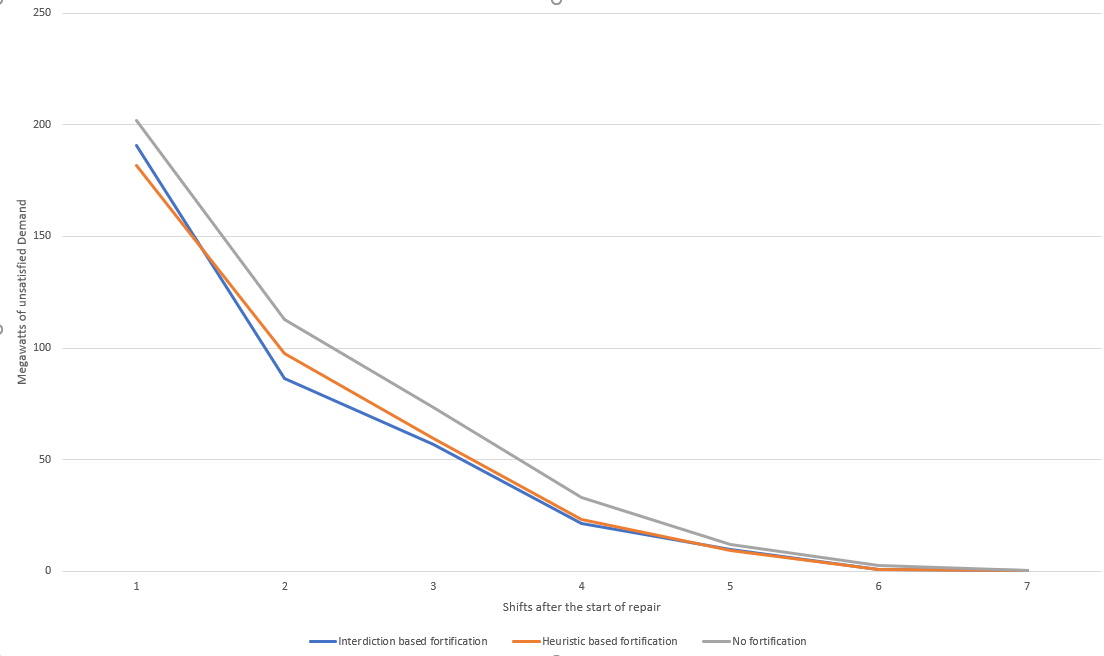
\includegraphics[width=.9\linewidth]{LowBudgetSpaghetti.png}
	\caption{Average repair curve for the tightened budget constraint}
\end{figure}
\begin{table}[htbp]
	\centering
		\caption{Expected unsatisfied demand by shift across resilience methods for a reduced hardening budget}
	\resizebox{\columnwidth}{!}{\begin{tabular}{|c|c|c|c|c|}
			\cline{1-5}
			Shift Number & Interdiction Based & Priority Heuristic Based & No Resilience & Perfect Information\\\hline
			1 & 192.2 & 184.8 & 201.4 & 127.6 \\\hline
			2 & 100.6 & 103.1 & 118.1 & 82.9 \\\hline
			3 & 64.7 & 61.8 & 76.0 & 43.0\\\hline
			4 & 25.6 & 25.4 & 35.7 & 19.5\\\hline
			5 & 12.1 & 10.6 & 13.3 & 5.12\\\hline
			6 & 1.85 & 1.21 & 2.75 & 0.83\\\hline
			7 & 0.22 & 0.22 & 0.33 & 0\\\hline
			total & 397.3 & 387.2 & 447.6 & 278.9\\\hline
	\end{tabular}}

	\label{time}
\end{table}

On the reduced budget, we see a similar conclusion to the higher budget example of resilience modeling when analyzing both Figure 4.6 and Table 4.3. In this case, the priority heuristic generates a slightly better solution in terms of both magnitude of initial drop and total lost load over the repair horizon. The reason for this is that interdiction based modeling can capture interactions between sets of elements. With only one node chosen, the impact of considering interactions rather than just heuristically choosing high priority elements is minimized. 

The conclusion from these two example studies into resilience is that the shape of the repair curves matter in terms of the end goal for resilient operations of power grids.  Changes in the curve shape leads to the difference in outcomes for the methods of choosing hardened elements on a power grid topology. Use of the repair curve captures both initial magnitude of damage as well as time to recovery when solving the optimal repair problem. As we see from comparing the interdiction based hardening to the priority heuristic solved hardening method, initial drop and time to resume nominal operations are not the only things that matter. Since interdiction based hardening is most frequently used in defense of a network against a directed attack and not a random event like a hurricane, it may not be the best tool for the job in planning resilience against a random event. We suspect this to be a place where probability based resilience methods based on hardening/fortifying the elements most likely to be damaged based on assessment of hurricane forecasts or some form of two step stochastic optimization to construct a resilience plan would be the best approach to take. 

